\section{Artificial Intelligence}
Artificial Intelligence (AI) refers to the ability of machines to exhibit "intelligence." Artificial intelligence research in computer science is defined as the study of "intelligent agents." An intelligent agent refers to any device that can perceive its environment and take actions that increase its chances of achieving a specific goal.\cite{russell2010artificial}. Initial research in this field was carried out by Alan Turing, the British Mathematician famous for breaking the Nazi's Enigma Cipher along with his team at Bletchley Park during World War 2. In 1938, Alan Turing developed his theory called "Turing Machines"\cite{Hodges+2015}, which was groundbreaking in its approach to define a new model for mathematical computation by defining an abstract machine, which consists of a tape and a set of arbitrary sequences called symbols, which are stored in discrete locations on the tape and can be later fetched by the machine. A Turing machine consists of a "head" and a finite set of states. The head is placed on one of the cells at any given time. During each step of the operation, the head reads the symbol present in the cell. Based on this symbol and the machine's current state, the machine writes a replacement symbol into the same cell and moves the head either one step left or right. Alternatively, it may stop the computation if necessary. To determine which symbol to write, which direction to move the head, or whether to halt, the machine refers to a finite table that specifies the correct action to take for each combination of the current state and symbol read. Turing opened the floodgates for computational theory and machine intelligence research with his work\cite{de2018turing}. Turing machines proved the possibility for computers to solve arbitrary problems by executing a finite set of operations and form basic reasoning abilities, hence inspiring researchers to conceptualize and work towards developing an "electronic brain." \\

In pursuit of emulating the human brain, researchers searched for inspiration from the biological world. The animal brain consists of a biological network (often called a neural circuit) that contains a large number of neurons, a type of nerve tissue that emits an electrical signal called neurotransmitters to other connected neurons through special connections called synapses. Neurons transmit signals to perform actions based on stimuli such as sensing, motor actions, etc. \cite{enwiki:1190738251}.
\begin{figure}[H]
    \centering
    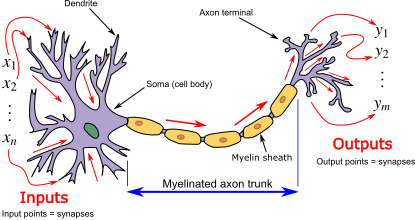
\includegraphics[width=\textwidth,height=5cm,keepaspectratio=true]{src/Images/Neuron3.png}
    \caption{
         Pictorial representation of a Neuron connection\cite{neuron_img}. 
    }
\end{figure}
\\ 
Incidentally, the first paper that describes a mathematical model for artificial neural networks also contains one of the earliest uses of the term AI was by McCullouch and Pitts. Their work proved the mathematical theorm behind artifical neurons. Artificial neural networks are now the backbone model of learning in today's popular machine learning models. Artificial neural networks were developed based on the biological model proposed by Hubel and Wiesel in 1959. During their research, they discovered two types of cells in the primary visual cortex, namely simple cells and complex cells. Many artificial neural networks are modeled as cascading systems of these cell types inspired by these biological observations. \cite{8259629}\\

Artificial neural networks (ANN) are composed of interconnected nodes that function similarly to neurons in biological neural circuits. Every ANN comprises of these core components: node character, network topology, and learning rules. The node character defines the flow and processing of signals, such as the number of inputs and outputs associated with the node, the weight assigned to each input and output, and the activation function. The network topology determines how the nodes are structured and connected. The learning rules define how the weights are initialized and adjusted. We will look at the topics in detail in Section 2.  \cite{livingstone2008artificial}

\begin{figure}[H]
    \centering
    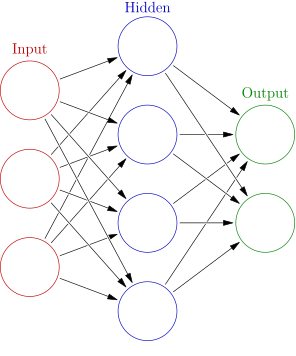
\includegraphics[width=\textwidth,height=7cm,keepaspectratio=true]{src/Images/Colored_neural_network.svg.png}
    \caption{
         Artificial Neural Network structure - signals are received at the input layer, processed in the hidden layers, and routed to the correct output node. Nodes are connected using weights \cite{ann_img}. 
    }
\end{figure}
\\

Machine learning (ML) is the subfield of artificial intelligence. Arthur Samuel, in 1959, defined machine learning as the "field of study that gives computers the ability to learn without being explicitly programmed.” The initial theories were more programmatic than probabilistic. Since then, ML approaches have advanced by borrowing many concepts from the domain of pattern recognition and computational learning theory in artificial intelligence. \cite{munoz2014machine}. \\

Machine learning explores the study and construction of algorithms that can learn from and make
predictions on data instead of being programmed with explicit instructions. Machine learning models are "trained" through sampling input data (also known as "training data"). For example, an ML model to detect forged cheques would be trained on data samples that include good, bad, and forged cheques. Machine learning is used in various applications where designing and programming explicit algorithms with good performance is difficult or unfeasible. ML approaches are further divided into three types of learning techniques based on the type of input data - Supervised Learning (labeled data), Unsupervised Learning (unlabeled data), and Semi-Supervised Learning.\cite{das2015applications}
\begin{figure}[H]
    \centering
    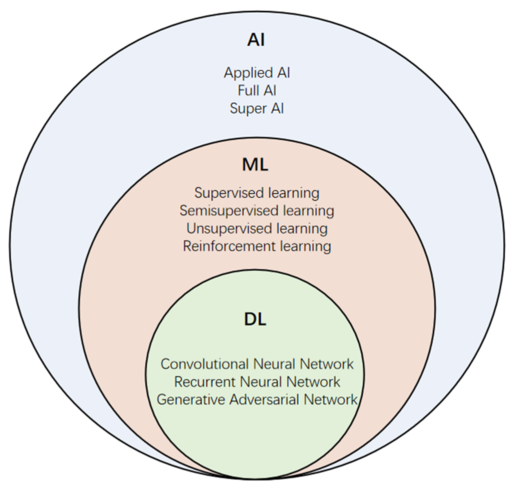
\includegraphics[width=\textwidth,height=6cm,keepaspectratio=true]{src/Images/ai_ml_dl.png}
    \caption{
      Relationship between AI, ML, and DL\cite{ai_ml_dl_img}
    }
\end{figure}
\\

One bottleneck that prevented advancements in ML research and development was the computationally expensive mathematical operations performed inside a neural network, such as large batch data ingestion, matrix multiplication, and transforms, which made it prohibitive for researchers to develop more complex ML algorithms using just a CPU. A processing core capable of high parallelization was required. A graphics processing unit (GPU) is a specialized processing unit, designed to rapidly manipulate data and alter memory locations. Their highly parallel structure makes them more efficient than general-purpose CPUs for algorithms where the processing of large blocks of data is done in parallel. The term GPU was popularized by Nvidia in 1999, who marketed the GeForce 256 as "the world's first GPU." GPUs played a critical role in the acceleration of AI research and production.\cite{8259629}

\begin{figure}[H]
    \centering
    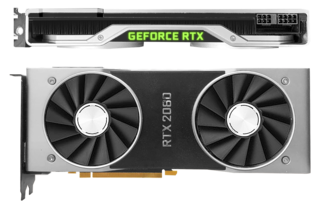
\includegraphics[width=\textwidth,height=4cm,keepaspectratio=true]{src/Images/RTX_2080FE.png}
    \caption{
         A modern GPU from Nvidia, popularly used for playing video games PC and video game consoles \cite{gpu_img}. 
    }
\end{figure}
\\

The term ”Deep Learning” (DL) was first introduced to Machine Learning (ML) in 1986 and later used for Artificial Neural Networks (ANN) in 2000 by Juergen Schmidhuber. Deep neural networks are an ML approach that involves adding multiple hidden layers between the input and output layers of an ANN. This allows for an extremely large number of possible connections, or "learnable weights," within the network. The hidden layers use a series of non-linear functions or filters to extract and transform features from the input. Each layer takes input from the previous layer and produces output for the next layer. As the network processes the input data, it builds increasingly complex pattern descriptors or features. These higher-level features are derived from lower-level features, creating a hierarchical representation of the input data. \cite{minar2018recent}. With the recent advances and commercial availability of GPUs, the field of research in deep neural networks and deep machine learning approaches has received much interest from the academic, commercial and government sectors.  
\begin{figure}[H]
    \centering
    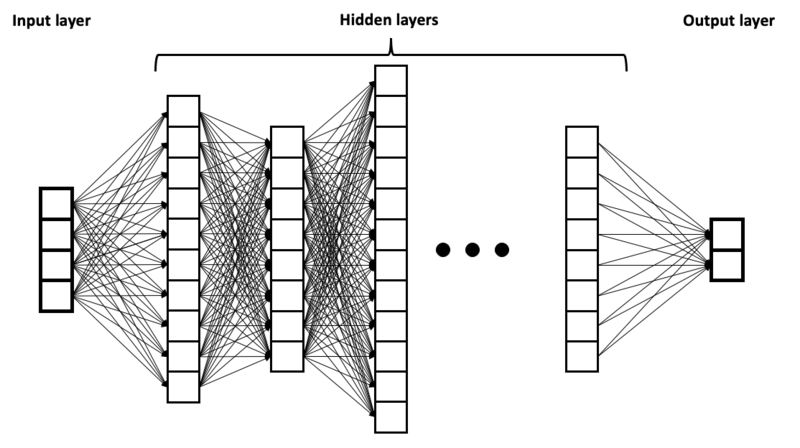
\includegraphics[width=\textwidth,height=6cm,keepaspectratio=true]{src/Images/Example_of_a_deep_neural_network.png}
    \caption{
    Example architecture of a deep neural network. \cite{dnn_img}. 
    }
\end{figure}
\\